% This is the Reed College LaTeX thesis template. Most of the work
% for the document class was done by Sam Noble (SN), as well as this
% template. Later comments etc. by Ben Salzberg (BTS). Additional
% restructuring and APA support by Jess Youngberg (JY).
% Your comments and suggestions are more than welcome; please email
% them to cus@reed.edu
%
% See http://web.reed.edu/cis/help/latex.html for help. There are a
% great bunch of help pages there, with notes on
% getting started, bibtex, etc. Go there and read it if you're not
% already familiar with LaTeX.
%
% Any line that starts with a percent symbol is a comment.
% They won't show up in the document, and are useful for notes
% to yourself and explaining commands.
% Commenting also removes a line from the document;
% very handy for troubleshooting problems. -BTS

% As far as I know, this follows the requirements laid out in
% the 2002-2003 Senior Handbook. Ask a librarian to check the
% document before binding. -SN

%%
%% Preamble
%%
% \documentclass{<something>} must begin each LaTeX document
\documentclass[12pt,twoside]{reedthesis}
% Packages are extensions to the basic LaTeX functions. Whatever you
% want to typeset, there is probably a package out there for it.
% Chemistry (chemtex), screenplays, you name it.
% Check out CTAN to see: http://www.ctan.org/
%%
\usepackage{graphicx,latexsym}
\usepackage{amsmath}
\usepackage{amssymb,amsthm}
\usepackage{longtable,booktabs,setspace}
\usepackage{chemarr} %% Useful for one reaction arrow, useless if you're not a chem major
\usepackage[hyphens]{url}
% Added by CII
\usepackage{hyperref}
\usepackage{lmodern}
\usepackage{float}
\floatplacement{figure}{H}
% End of CII addition
\usepackage{rotating}

% Next line commented out by CII
%%% \usepackage{natbib}
% Comment out the natbib line above and uncomment the following two lines to use the new
% biblatex-chicago style, for Chicago A. Also make some changes at the end where the
% bibliography is included.
%\usepackage{biblatex-chicago}
%\bibliography{thesis}


% Added by CII (Thanks, Hadley!)
% Use ref for internal links
\renewcommand{\hyperref}[2][???]{\autoref{#1}}
\def\chapterautorefname{Chapter}
\def\sectionautorefname{Section}
\def\subsectionautorefname{Subsection}
% End of CII addition

% Added by CII
\usepackage{caption}
\captionsetup{width=5in}
% End of CII addition

% \usepackage{times} % other fonts are available like times, bookman, charter, palatino

% Syntax highlighting #22

% To pass between YAML and LaTeX the dollar signs are added by CII
\title{Proto-Solutrean lithic technology of Western Iberia: sites of Vale Boi and Lapa do Picareiro}
\author{Joana Belmiro}
% The month and year that you submit your FINAL draft TO THE LIBRARY (May or December)
\date{May 2020}
\division{Faculdade de Ciências Humanas e Sociais}
\advisor{João Cascalheira}
\institution{Universidade do Algarve}
\degree{Mestrado em Arqueologia}
%If you have two advisors for some reason, you can use the following
% Uncommented out by CII
% End of CII addition

%%% Remember to use the correct department!
\department{Arqueologia}
% if you're writing a thesis in an interdisciplinary major,
% uncomment the line below and change the text as appropriate.
% check the Senior Handbook if unsure.
%\thedivisionof{The Established Interdisciplinary Committee for}
% if you want the approval page to say "Approved for the Committee",
% uncomment the next line
%\approvedforthe{Committee}

% Added by CII
%%% Copied from knitr
%% maxwidth is the original width if it's less than linewidth
%% otherwise use linewidth (to make sure the graphics do not exceed the margin)
\makeatletter
\def\maxwidth{ %
  \ifdim\Gin@nat@width>\linewidth
    \linewidth
  \else
    \Gin@nat@width
  \fi
}
\makeatother

\renewcommand{\contentsname}{Table of Contents}
% End of CII addition

\setlength{\parskip}{0pt}

% Added by CII

\providecommand{\tightlist}{%
  \setlength{\itemsep}{0pt}\setlength{\parskip}{0pt}}

\Acknowledgements{

}

\Dedication{

}

\Preface{

}

\Abstract{
The present study aims to answer the question: what impact did the Heinrich 2 event have on the technological organization of human communities, at the onset of the last glacial maximum, in south western Iberia? The impact of this event on the Gravettian-Soluttrean transition has been previously suggested (Bradtmöller, Pastoors, Weninger, \& Weniger, 2012). However, the existing models do not consider the Proto-Solutrean technocomplex as an individual phase for this transition (Cascalheira \& Bicho, 2013).

\par

To address this question, this study analysed the lithic assemblages from Vale Boi (south Portugal) and Lapa do Picareiro (central Portugal). We aimed to understand the technological patterns and raw material exploitation during the Proto-Solutrean, and test the existing models with assemblages from recently excavated sites, while expanding the geographic range.

The analysis followed a technologic and morphologic attribute approach. The retrieved data was then analysed through descritive statistics in R environment.

Results show the existence of two occupations within the assemblages. The first, with high frequency of quartz use for bladelet production, seems to reflect a Terminal Gravettian horizon. The appearance of Vale Comprido technology and lower quartz frequencies in a second moment in Vale Boi seem to represent a Proto-Solutrean occupation. The second horizon in Lapa do Picareiro, with the presence of Vale Comprido-like technology but with low flattening ratios may be attributed to a Proto-Solutrean or an Early Solutrean occupation.

The Terminal Gravettian and Proto-Solutrean seem to be chronologically different phases, in concordance with the Three-Phase model for the Proto-Solutrean (Zilhão, 1997). The similarities between Vale Boi and the Estremadura may be explained by the expansion of social networks (Cascalheira \& Bicho, 2013). Associated with the dominance of different technologic patterns and intensive use of quartz, we may understand these horizons as a moment of cultural reorganization, onset by environmental pressures.

Keywords: Upper Paleolithic; Attribute analysis; Raw material exploitation; Climatic changes.
}

\Resumo{
O objetivo desta tese é responder à seguinte pergunta: que impacto teve o evento climático Heinrich 2 (HE 2) na organização tecnológica das comunidades de caçadores-recolectores no início do último máximo glacial (LGM), no sudoeste peninsular?

\par

Esta questão está intimamente ligada ao entendimento de certos eventos climáticos abruptos, tais como os eventos de Heinrich ou os Estados Glaciares, com a substituição de culturas ao longo do Paleolítico Superior. Um destes momentos de substituição correlaciona a passagem do Gravetense para o Solutrense com o evento HE 2 e com o Estádio Glacial 3, possivelmente sobreposta pelo LGM. Neste paradigma, as mudanças climáticas desencadeiam mudanças sociais, através do colapso de tradições que depois são reorganizadas, de forma a corresponder às novas condições ambientais e paisagísticas. No entanto, nos modelos existentes, o Proto-Solutrense não surge como um tecnocomplexo individualizado, existindo assim uma lacuna no entendimento atual do processo de transição entre os dois horizontes culturais supramencionados.

O Proto-Solutrense, representado sobretudo na Estremadura Portuguesa, é entendido como um tecnocomplexo de transição, ocorrendo entre os 26 000 cal BP e 25 400 cal BP, e caracterizado por mudanças na tecnologia e preferência de matérias-primas, existindo dois modelos para a sua evolução: modelo em duas etapas; e modelo em três etapas.

O modelo em duas etapas considera a existência do Gravetense Final e Proto-Solutrense, caracterizado pelo uso intensivo de quartzo e estratégias de produção para obtenção de lamelas em núcleos carenados e obtenção de suportes convergentes para pontas de Vale Comprido, sendo, no entanto, caracterizado por uma alta variabilidade interna. O modelo em três etapas consiste na evolução do Gravetense Final para uma etapa intermédia (no modelo das duas etapas considerada uma fácies funcional do Proto-Solutrense), caracterizada pelo uso intensivo do quartzo, estratégias de redução para obtenção de lamelas em núcleos carenados, seguida de uma fase Proto-Solutrense caracterizada pela diminuição do uso do quartzo e estratégias de redução para obtenção de suportes convergentes para pontas de Vale Comprido.
O conhecimento atual do Proto-Solutrense apresenta-se truncado, no entanto, pela antiguidade de algumas escavações e a sua restrição geográfica à Estremadura Portuguesa.

De forma a responder à questão supramencionada, assim como contribuir para o conhecimento do Proto-Solutrense no sudoeste Peninsular, foram analisados os conjuntos líticos de Vale Boi (sul de Portugal) e Lapa do Picareiro (Portugal central), ambos escavados nos últimos 20 anos com recurso a estações totais. Esta análise teve a finalidade de entender os padrões tecnológicos e de exploração do território durante o Proto-Solutrense, através dos seguintes objetivos: 1) entender e explicar os padrões tecnológicos e de preferência de matérias-primas intra-sítio; 2) estabelecer paralelos entre os dois sítios; 3) comparar estes resultados com os obtidos em outros sítios com conjuntos Proto-Solutrenses, sobretudo da Estremadura.

A análise seguiu uma abordagem de atributos tecnológicos e morfológicos, seguida de uma fase de tratamento estatístico através de duas metodologias: estatística descritiva e multivariada, ambas efetuadas em ambiente R. A análise multivariada segue a metodologia já descrita noutros trabalhos (Tostevin 2012; Scerri et al.~2014), e que passa pelo agrupamento de vários atributos em domínios tecnológicos, cada qual representando uma escolha do talhador(a) em alturas chave do talhe, de forma a reduzir a variabilidade interna dos conjuntos.

Palavras-chave: Paleolítico Superior; Padrões tecnológicos; Exploração de matérias-primas.
}

	\usepackage[T1]{fontenc}
\usepackage[utf8]{inputenc}
	\usepackage{booktabs}
\usepackage{longtable}
\usepackage{array}
\usepackage{multirow}
\usepackage{wrapfig}
\usepackage{float}
\usepackage{colortbl}
\usepackage{pdflscape}
\usepackage{tabu}
\usepackage{threeparttable}
\usepackage{threeparttablex}
\usepackage[normalem]{ulem}
\usepackage{makecell}
\usepackage{xcolor}
% End of CII addition
%%
%% End Preamble
%%
%
\begin{document}

% Everything below added by CII
  \maketitle

\frontmatter % this stuff will be roman-numbered
%\pagestyle{empty} % this removes page numbers from the frontmatter


  \begin{abstract}
    The present study aims to answer the question: what impact did the Heinrich 2 event have on the technological organization of human communities, at the onset of the last glacial maximum, in south western Iberia? The impact of this event on the Gravettian-Soluttrean transition has been previously suggested (Bradtmöller, Pastoors, Weninger, \& Weniger, 2012). However, the existing models do not consider the Proto-Solutrean technocomplex as an individual phase for this transition (Cascalheira \& Bicho, 2013).
    
    \par
    
    To address this question, this study analysed the lithic assemblages from Vale Boi (south Portugal) and Lapa do Picareiro (central Portugal). We aimed to understand the technological patterns and raw material exploitation during the Proto-Solutrean, and test the existing models with assemblages from recently excavated sites, while expanding the geographic range.
    
    The analysis followed a technologic and morphologic attribute approach. The retrieved data was then analysed through descritive statistics in R environment.
    
    Results show the existence of two occupations within the assemblages. The first, with high frequency of quartz use for bladelet production, seems to reflect a Terminal Gravettian horizon. The appearance of Vale Comprido technology and lower quartz frequencies in a second moment in Vale Boi seem to represent a Proto-Solutrean occupation. The second horizon in Lapa do Picareiro, with the presence of Vale Comprido-like technology but with low flattening ratios may be attributed to a Proto-Solutrean or an Early Solutrean occupation.
    
    The Terminal Gravettian and Proto-Solutrean seem to be chronologically different phases, in concordance with the Three-Phase model for the Proto-Solutrean (Zilhão, 1997). The similarities between Vale Boi and the Estremadura may be explained by the expansion of social networks (Cascalheira \& Bicho, 2013). Associated with the dominance of different technologic patterns and intensive use of quartz, we may understand these horizons as a moment of cultural reorganization, onset by environmental pressures.
    
    Keywords: Upper Paleolithic; Attribute analysis; Raw material exploitation; Climatic changes.
  \end{abstract}
  \begin{resumo}
    O objetivo desta tese é responder à seguinte pergunta: que impacto teve o evento climático Heinrich 2 (HE 2) na organização tecnológica das comunidades de caçadores-recolectores no início do último máximo glacial (LGM), no sudoeste peninsular?
    
    \par
    
    Esta questão está intimamente ligada ao entendimento de certos eventos climáticos abruptos, tais como os eventos de Heinrich ou os Estados Glaciares, com a substituição de culturas ao longo do Paleolítico Superior. Um destes momentos de substituição correlaciona a passagem do Gravetense para o Solutrense com o evento HE 2 e com o Estádio Glacial 3, possivelmente sobreposta pelo LGM. Neste paradigma, as mudanças climáticas desencadeiam mudanças sociais, através do colapso de tradições que depois são reorganizadas, de forma a corresponder às novas condições ambientais e paisagísticas. No entanto, nos modelos existentes, o Proto-Solutrense não surge como um tecnocomplexo individualizado, existindo assim uma lacuna no entendimento atual do processo de transição entre os dois horizontes culturais supramencionados.
    
    O Proto-Solutrense, representado sobretudo na Estremadura Portuguesa, é entendido como um tecnocomplexo de transição, ocorrendo entre os 26 000 cal BP e 25 400 cal BP, e caracterizado por mudanças na tecnologia e preferência de matérias-primas, existindo dois modelos para a sua evolução: modelo em duas etapas; e modelo em três etapas.
    
    O modelo em duas etapas considera a existência do Gravetense Final e Proto-Solutrense, caracterizado pelo uso intensivo de quartzo e estratégias de produção para obtenção de lamelas em núcleos carenados e obtenção de suportes convergentes para pontas de Vale Comprido, sendo, no entanto, caracterizado por uma alta variabilidade interna. O modelo em três etapas consiste na evolução do Gravetense Final para uma etapa intermédia (no modelo das duas etapas considerada uma fácies funcional do Proto-Solutrense), caracterizada pelo uso intensivo do quartzo, estratégias de redução para obtenção de lamelas em núcleos carenados, seguida de uma fase Proto-Solutrense caracterizada pela diminuição do uso do quartzo e estratégias de redução para obtenção de suportes convergentes para pontas de Vale Comprido.
    O conhecimento atual do Proto-Solutrense apresenta-se truncado, no entanto, pela antiguidade de algumas escavações e a sua restrição geográfica à Estremadura Portuguesa.
    
    De forma a responder à questão supramencionada, assim como contribuir para o conhecimento do Proto-Solutrense no sudoeste Peninsular, foram analisados os conjuntos líticos de Vale Boi (sul de Portugal) e Lapa do Picareiro (Portugal central), ambos escavados nos últimos 20 anos com recurso a estações totais. Esta análise teve a finalidade de entender os padrões tecnológicos e de exploração do território durante o Proto-Solutrense, através dos seguintes objetivos: 1) entender e explicar os padrões tecnológicos e de preferência de matérias-primas intra-sítio; 2) estabelecer paralelos entre os dois sítios; 3) comparar estes resultados com os obtidos em outros sítios com conjuntos Proto-Solutrenses, sobretudo da Estremadura.
    
    A análise seguiu uma abordagem de atributos tecnológicos e morfológicos, seguida de uma fase de tratamento estatístico através de duas metodologias: estatística descritiva e multivariada, ambas efetuadas em ambiente R. A análise multivariada segue a metodologia já descrita noutros trabalhos (Tostevin 2012; Scerri et al.~2014), e que passa pelo agrupamento de vários atributos em domínios tecnológicos, cada qual representando uma escolha do talhador(a) em alturas chave do talhe, de forma a reduzir a variabilidade interna dos conjuntos.
    
    Palavras-chave: Paleolítico Superior; Padrões tecnológicos; Exploração de matérias-primas.
  \end{resumo}
  \hypersetup{linkcolor=black}
  \setcounter{tocdepth}{2}
  \tableofcontents

  \listoftables

  \listoffigures


\mainmatter % here the regular arabic numbering starts
\pagestyle{fancyplain} % turns page numbering back on

\hypertarget{if-you-have-more-two-advisors-un-silence-line-7}{%
\chapter{If you have more two advisors, un-silence line 7}\label{if-you-have-more-two-advisors-un-silence-line-7}}

Placeholder

\hypertarget{introduction}{%
\chapter{Introduction}\label{introduction}}

The replacement of the Gravettian technocomplex by the Solutrean, impacted by adverse climatic conditions during the Heinrich Event 2 (HE2), continues to be an essential topic for understanding the Upper Paleolithic and Human adaptations to climatic changes. The Proto-Solutrean is, in this topic, an essential piece to understand how hunter-gatherer communities adapted, reinvented and destroyed their social and technologic organization which eventually allowed the development of the Solutrean. However, most of what is known for this technocomplex is still geographically constricted and lacking good chronological markers (Cascalheira \& Bicho, 2013), which hampers the understanding of the Proto-Solutrean itself and its role in the Gravettian-Solutrean transition.

By understanding the need to better comprehend the Proto-Solutrean and how adverse climate impacted these communities, this study aims to answer the following question: what impact did the HE 2 have on the technological organization of human communities, at the onset of the last glacial maximum, in south western Iberia? To do so, this study will analyse the lithic terminal gravettian/proto-solutrean assemblages of two recently excavated sites with resource to total stations, Vale Boi (south of Portugal) and Lapa do Picareiro (central Portugal).

To answer this question, we aim to accomplish the following goals:
\begin{itemize}
\item
  Understand the technological organization of layers 5/4E of Vale Boi and U to Middle T from Lapa do Picareiro, by characterizing their technological patterns, reduction sequences and raw material use/preference patterns. The results will then be compared with the existing data from other proto-solutrean assemblages, mostly from the Estremadura Portuguesa.
\item
  Identify possible terminal gravettian horizons or facies within the proto-solutrean occupations in Vale Boi and Lapa do Picareiro and their chronologies.
\item
  Test the proto-solutrean transition models (Two-phase and Three-phase) developed through results from the Estremadura to understand which model best explains the transition between the Final Gravettian to the Proto-Solutrean, and whether the model may be applied to other geographic areas outside of the Estremadura.
\end{itemize}
By accomplishing these goals, through the use of new data resulting from recent excavations, with good chronological markers and a wider geographic range (south of Portugal), we hope to contribute to the understanding of the Proto-Solutrean and the Gravettian-Solutrean transition in western Iberia.

The present thesis is organized in 7 chapters:
\begin{itemize}
\item
  Chapter 2, where we will discuss the impact of climatic changes on culture replacement, especially during the HE 2, describe the paleoclimate during this event and finally describe the Proto-Solutrean and its technological characteristics.
\item
  Chapter 3 which will introduce the archaeological sites used in the study with a brief description of their location and geological context, followed by an overview of excavation works, excavation methodology, human occupation through the several areas and layers, then focusing on the layers associated with terminal gravettian/proto-solutrean horizons.
\item
  Chapter 4, where we will overview the methodology employed in both the lithic and data analysis.
\item
  Chapter 5 which will consist on the description of the results obtained through the analysis of the assemblages from Vale Boi and Lapa do Picareiro, respectively. This will be organized by assemblage description, raw materials and technology.
\item
  Chapter 6 will focus on the discussion of the results presented in the previous chapter, comparing them to other results from proto-solutrean assemblages, mostly from the Portuguese Estremadura. In this chapter we will also discuss problematics which relate to the goals abovementioned.
\item
  Chapter 9 will consist of this study's conclusions, systematizing the analysis interpretations and discussion.
\end{itemize}
\hypertarget{human-adaptations-at-the-start-of-the-last-glacial-maximum}{%
\chapter{Human adaptations at the start of the last glacial maximum}\label{human-adaptations-at-the-start-of-the-last-glacial-maximum}}

Placeholder

\hypertarget{paleoclimate-paleoenvironment-and-human-adaptation-models}{%
\section{Paleoclimate, paleoenvironment and human adaptation models}\label{paleoclimate-paleoenvironment-and-human-adaptation-models}}

\hypertarget{proto-solutrean-origins-and-the-portuguese-model}{%
\section{Proto-Solutrean: origins and the Portuguese model}\label{proto-solutrean-origins-and-the-portuguese-model}}

\hypertarget{archaeological-sites}{%
\chapter{Archaeological sites}\label{archaeological-sites}}

Placeholder

\hypertarget{location-and-geological-context}{%
\section{Location and geological context}\label{location-and-geological-context}}

\hypertarget{vale-boi}{%
\subsection{Vale Boi}\label{vale-boi}}

\hypertarget{lapa-do-picareiro}{%
\subsection{Lapa do Picareiro}\label{lapa-do-picareiro}}

\hypertarget{research-history-stratigraphy-and-human-occupation}{%
\section{Research history, stratigraphy and human occupation}\label{research-history-stratigraphy-and-human-occupation}}

\hypertarget{vale-boi-1}{%
\subsection{Vale Boi}\label{vale-boi-1}}

\hypertarget{slope}{%
\subsubsection{Slope}\label{slope}}

\hypertarget{shelter}{%
\subsubsection{Shelter}\label{shelter}}

\hypertarget{terrace}{%
\subsubsection{Terrace}\label{terrace}}

\hypertarget{lapa-do-picareiro-1}{%
\subsection{Lapa do Picareiro}\label{lapa-do-picareiro-1}}

\hypertarget{levels-u-to-middle-t}{%
\subsubsection{Levels U to middle T}\label{levels-u-to-middle-t}}

\hypertarget{excavation-methodology}{%
\section{Excavation methodology}\label{excavation-methodology}}

\hypertarget{methodology}{%
\chapter{Methodology}\label{methodology}}

\hypertarget{attribute-analysis}{%
\section{Attribute analysis}\label{attribute-analysis}}

In order to understand the multiple causes for lithic variation, such as raw material properties or local adaptations, researchers are increasingly adopting sophisticated methods of lithic analysis, then linking that data to explanatory theories of human behavior (Scerri, Groucutt, Jennings, \& Petraglia, 2014). Examples of such studies are those by Brantingham \& Kuhn (2001), who apply a geometric and mathematical model to understand Levallois core morphology, or Dibble \& Rezek (2009), that through platform attributes try to understand flake variability.

Despite the existence of several different concepts in quantitative analysis, the basic units of analysis continue to be the technological attributes (Scerri et al., 2014). These attributes are measurable (e.g.~length, width or thickness) and observable (e.g.~platform type or cross section type) proxies for understanding lithic shape and production methods (Inizan, Reduron-Ballinger, Roche, \& Tixier, 1999). Following certain paradigms, like referred above, they can be quantified in different ways, such as diversity, mechanical relationships, shapes and reduction sequences, in order to better understand lithic assemblages (Scerri et al., 2014) and the role that lithics played in past adaptations over time and space (Foley \& Lahr, 2003).

The application of attribute analysis does have some caveats, linked mainly to how such attributes are interpreted by the archaeologist and their actual contribution to the understanding of an assemblage's variability (Dibble, 2008; Scerri et al., 2014). Nonetheless, this approach was chosen for the present study, for the recognized benefits such as flexibility (resolution and amount of information recovered) and broadness of utility (Tostevin, 2012).

The application of this methodology, which aims to recover morphological and metrical attributes of technological classes, has been present in pre-historical European contexts since the 1970s (Bicho, 1992). In Portugal, this methodology has been applied by Bicho (1992) who characterized Rio Maior's Upper Paleolithic lithic assemblages, Zilhão (1997) for the Upper Paleolithic archaeological sites of Estremadura or Almeida (2000), who associated attribute analysis with refitting to characterize the Terminal Gravettian of the Estremadura.

Regarding the latter approach, refitting, despite allowing a precise description of the sequences of knapping operations from the beginning of the knapping sequence to the final desired products, has too many caveats for its application in the present study (Tostevin, 2012). Often, assemblages may not gather the requisites which are necessary for the application of this methodology such as adequate contextual preservation or presence of complete in situ knapping sequences or the investigators may not have either the time or space for it. Additionally, one or two totally refitted nodules may or may not be representative of the dominant operative sequence, especially in situations where there is high internal variability (Tostevin, 2012). Regarding the sites in this study, Vale Boi's layer 5 and 4E assemblage shows a high degree of variability, and Lapa do Picareiro's U to middle T assemblage shows a truncated reduction sequence (due to site function and high altitude location). Given the aforementioned problematics, the present study used only an attribute analysis approach without refits.

All artefacts and their technological and morphological attributes were recorded using two different databases, thus dividing the analysis in two phases: basic and complete attribute-based analysis.
In both cases, data collection was done through E4, a software developed by Dibble and McPherron (2003), available for download at \url{http://www.oldstoneage.com/software/default.shtml}. The software allows the user to program a database file which filters variables through conditions, defined by previous choices and attributes, which allows for better control of the database and homogeneous results. After recording, all information is gathered in one single database in an Access type output.
The basic analysis (appendix X) was applied to all of Vale Boi's quartz artefacts (layers 5 and 4E), since all lithics from the same assemblage in other raw-materials (e.g.~chert and greywacke) had been previously analyzed with the same database (\emph{vide}, Belmiro, 2018). This database consists of a reduced set of variables which allow for the general classification of metric and morphologic characteristics of the artefacts, as well as the identification of raw material preference and preferential use. These main variables were: 1) raw material; 2) technological class, following the traditional criteria for lithic technological analysis (Andrefsky \& Andrefsky Jr, 1998; Bicho \& Jorge, 2011; Debénath \& Dibble, 1994; Inizan et al., 1999); percentage of cortex (Bicho \& Jorge, 2011); weight and mesial thickness, maximum width and maximum length. Retouched pieces were classified into wider groups regarding their morphologies and retouch type, following the typologies defined by Sonneville-Bordes \& Perrot (1956), adapted by Zilhão (1997) for the Portuguese Estremadura.

The complex analysis was applied to Vale Boi complete cores, debitage products and retouched pieces. Only pieces which were complete were chosen for this stage for two main reasons: 1) the collection is well preserved, with high percentages of complete cores and blanks (\textasciitilde80\%), guaranteeing that the sample is representative; 2) only complete pieces gather all the necessary attributes for a thorough analysis. The same database was applied to the whole assemblage of Lapa do Picareiro, given its small sample size.

The several attributes analysed in this database follow those present in specialized literature, such as Brézillon (1968) and Tixier \& Inizian (1980), paired with the methodologies used in Upper Paleolithic lithic attribute analysis works, such as Bicho (1992), Zilhão (1997) or Almeida (2000).

The complete Data Dictionary with all variables, attributes, values and description, with reference to the consulted literature can be found in Appendix X.

Regarding cores, the following variables were registered: section, type of platform and number of platforms, core morphology, following the types defined by Bicho (1992) and Brézillon (1968), percentage of cortex, types and number of extracted products (with maximum, proximal, mesial and distal measurements of the final extraction) and reason for abandonment. When cores showed more than one face, a dominant debitage face was established, which allowed for the orientation of the artefact and recording of some of the variables (e.g.~measurements of final extraction).

For debitage products and EMNP, their technological class, morphology, section and profile were recorded, following the definitions by Zilhão (1997). Other determined attributes were the presence of lipping and type of platform, according to Inizan et al. (1999), percentage of cortex and amount of dorsal extractions (\textgreater{} 5 mm). Retouched pieces were classified into wide groups as applied in the simple database, following once again the typologies defined by Sonneville-Bordes \& Perrot (1956), adapted by Zilhão (1997) for the Portuguese Estremadura.

Regarding the technological classes, the values recorded were core, blank, retouched piece and core preparation product following traditional analysis criteria (Andrefsky \& Andrefsky Jr, 1998; Bicho \& Jorge, 2011; Debénath \& Dibble, 1994; Inizan et al., 1999), but collapsing both flakes and elongated blanks in a single category. The difference between flake and elongated blank is traditionally defined by a ratio between length and width measurements. Elongated blanks are defined as products whose length is equal or greater than twice their width (Bicho \& Jorge, 2011; Tixier \& Inizian, 1980). Very frequently, this ratio is blurred, resulting in elongated flakes or short elongated blanks, which may result in incorrect classifications. In understanding both flakes and elongated blanks as a whole, without prior classification, and using the measurements recorded if needed, we achieve the same results without the need to find classification mistakes and without delving into typologies which may not have any real technological significance. The same methodology was applied regarding the definition of bladelet and blade. As traditionally defined, bladelets are elongated blanks with maximum width of 12 mm, whereas blades are elongated blanks with more than 12 mm of width or more than 50 mm of length (Tixier, 1963). For the present study, this typological differentiation was not applied during the analysis, since it may be achieved, if needed, with the recorded measurements.

The measurements were registered equally for debitage products and cores as shown in figure \ref{fig:metric}, which included the measurement of the platform angle according to Dibble (1997), with the goal of understanding platform morphology, which, according to the author, may offer a better understanding of lithic technological variability. In this case, the variation in exterior platform angle, platform depth and angle of blow seem to explain flake size, and the variation of the exterior platform angle seems to have an impact on flake shape as well, both of which have implications in understanding the employment of different strategies for preferential size of blank products (Dibble, 1997; Dibble \& Rezek, 2009; Leader, Abdolahzadeh, Lin, \& Dibble, 2017; Lin, Rezek, Braun, \& Dibble, 2013).
\begin{figure}
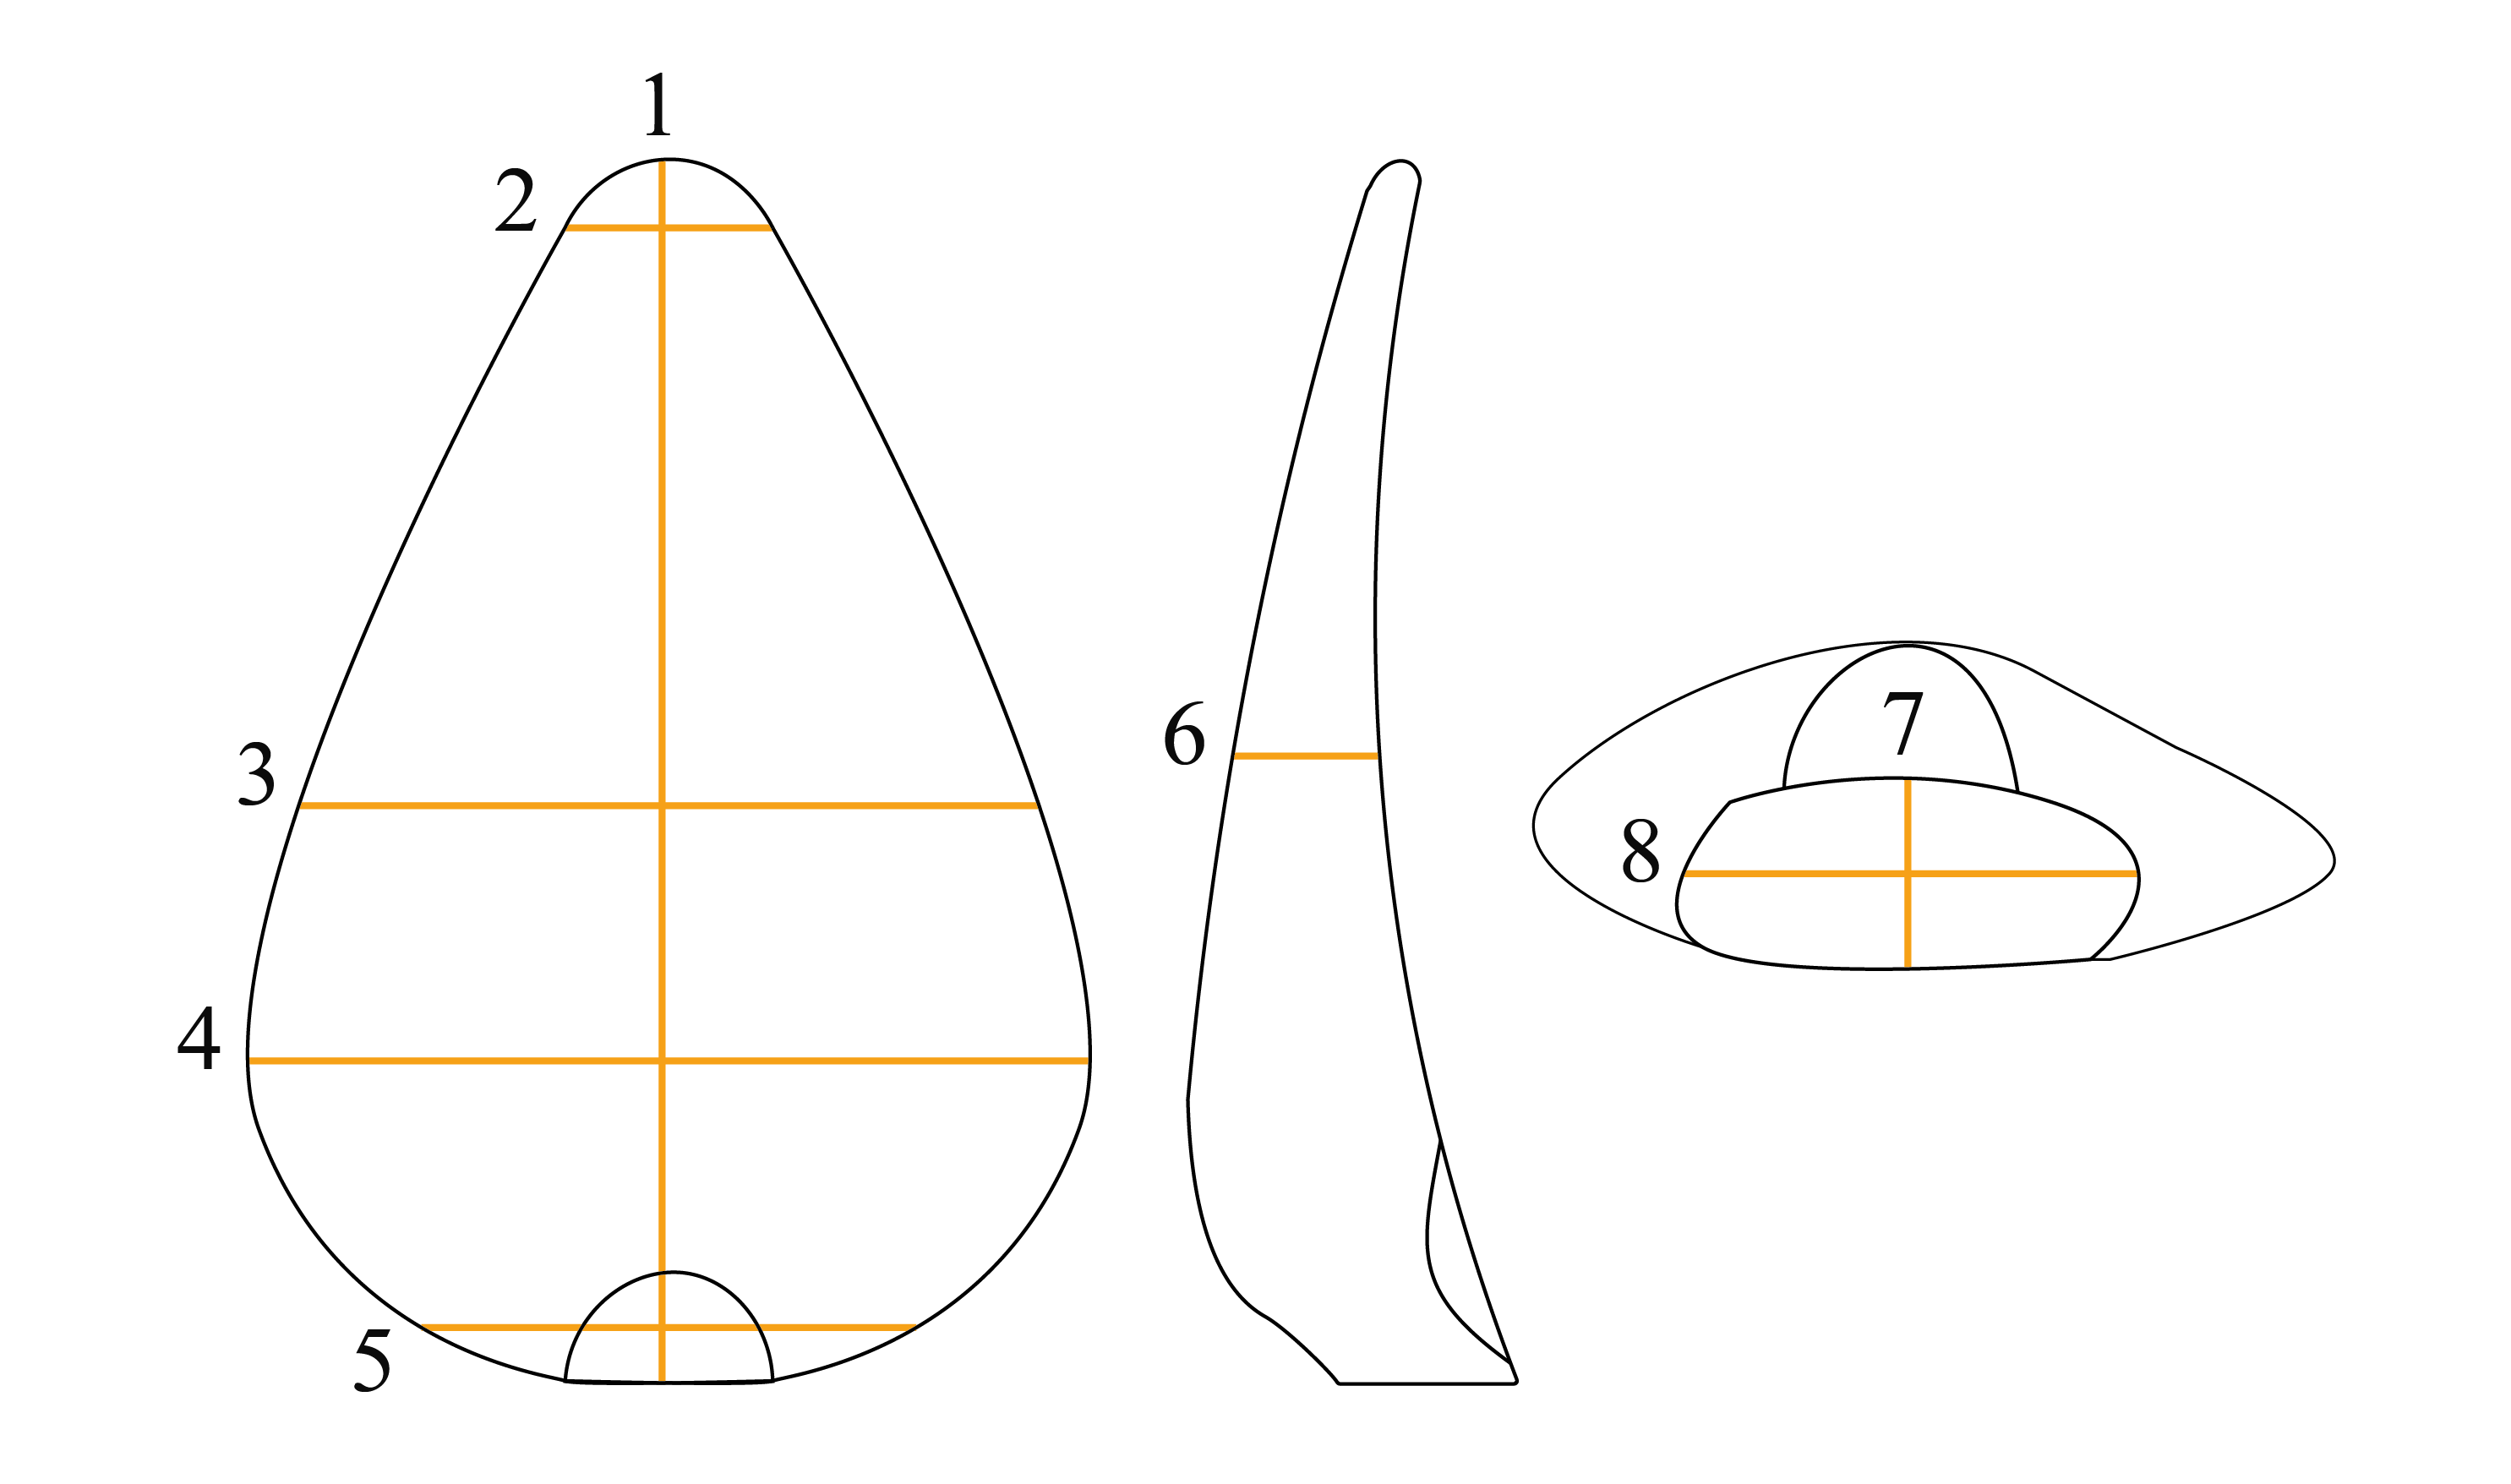
\includegraphics[width=1\linewidth]{figure/Metrics-01} \caption{Registered measurements scheme for debitage products and cores. Legend: 1- Maximum length; 2- Distal width; 3- Mesial width; 4- Maximum width; 5- Proximal width; 6- Mesial thickness; 7- Platform thickness; 8- Platform width.}\label{fig:metric}
\end{figure}
Finally, although raw material had been previously analysed in the simple attribute analysis, quartz artefacts were subdivided regarding raw material quality. When analysing the quartz lithic collection, it was apparent that fracture patterns and product morphology differed greatly between quartz and other raw materials and even within types of quartz. In fact, it is understood that applying the same analysis variables to all raw materials, especially quartz, may not be the most appropriate methodology, since different technological solutions might be applied to materials which react differently to knapping (Beardsell, 2013). Despite this, creating a different database or establishing different analysis attributes for quartz would result in different issues and problems that would require further testing and experimenting. Thus, in order to understand possible preferential uses or mechanical constraints of quartz, this raw material was analysed with the same attributes as other raw materials, but further classified regarding its quality. In fact, Almeida (2000) stated that, for the Terminal Gravettian, raw material quality, namely the quartz, resulted in specific behaviours and different technological patterns. By defining quartz quality and understanding the collection through this added variable, it was our goal to better comprehend the cultural horizon in its fullest, and allow comparison to other studies, in which similar variables were considered.

Quartz quality was defined by grain size: coarse quality was applied to every quartz artefact that displayed large and visible grains (\textgreater0.5 mm); medium quality was applied whenever the grains were visible but small (\textless0.5 mm); fine quality was defined by the absence of visible grains; and rock crystal was applied whenever there was the absence of visible grains, but where the minerals were translucent.

\hypertarget{data-analysis}{%
\section{Data analysis}\label{data-analysis}}

After data collection, the databases, for both Vale Boi and Lapa do Picareiro, were imported into R environment, where the information was processed through the creation of descriptive statistical analysis. This and the writing of this thesis were done in RStudio, an open source integrated development environment (IDE) for R, which can be downloaded at \url{https://rstudio.com}, also with resource to RMarkdown, which allows the production of fully reproducible documents (downloaded at \url{https://rmarkdown.rstudio.com}) Following the goal for transparent science and reproducible results, the script programmed for this analysis, as well as all the raw data used can be consulted online through the following DOI (\url{https://osf.io/7hz52/}). To produce those files the procedures described by Marwick (2017) for the creation of research compendiums to enhance the reproducibility of research were followed. A list with all R packages used in the analysis is also present in Appendix X. To enable maximum re-use, the code is released under the MIT license, data as CC-0, and figures as CC-BY (for more information see, Marwick, Boettiger, \& Mullen, 2018).

\hypertarget{results}{%
\chapter{Results}\label{results}}

Placeholder

\hypertarget{assemblages}{%
\section{Assemblages}\label{assemblages}}

\hypertarget{vale-boi-2}{%
\subsection{Vale Boi}\label{vale-boi-2}}

\hypertarget{lapa-do-picareiro-2}{%
\subsection{Lapa do Picareiro}\label{lapa-do-picareiro-2}}

\hypertarget{raw-materials}{%
\section{Raw materials}\label{raw-materials}}

\hypertarget{vale-boi-3}{%
\subsection{Vale Boi}\label{vale-boi-3}}

\hypertarget{quartz}{%
\subsubsection{Quartz}\label{quartz}}

\hypertarget{chert}{%
\subsubsection{Chert}\label{chert}}

\hypertarget{greywacke}{%
\subsubsection{Greywacke}\label{greywacke}}

\hypertarget{dolerite}{%
\subsubsection{Dolerite}\label{dolerite}}

\hypertarget{chalcedony}{%
\subsubsection{Chalcedony}\label{chalcedony}}

\hypertarget{lapa-do-picareiro-3}{%
\subsection{Lapa do Picareiro}\label{lapa-do-picareiro-3}}

\hypertarget{quartz-1}{%
\subsubsection{Quartz}\label{quartz-1}}

\hypertarget{chert-1}{%
\subsubsection{Chert}\label{chert-1}}

\hypertarget{technological-analysis}{%
\section{Technological analysis}\label{technological-analysis}}

\hypertarget{cores}{%
\subsection{Cores}\label{cores}}

\hypertarget{vale-boi-4}{%
\subsubsection{Vale Boi}\label{vale-boi-4}}

\hypertarget{lapa-do-picareiro-4}{%
\subsubsection{Lapa do Picareiro}\label{lapa-do-picareiro-4}}

\hypertarget{core-maintenance-products}{%
\subsection{Core maintenance products}\label{core-maintenance-products}}

\hypertarget{flakes}{%
\subsection{Flakes}\label{flakes}}

\hypertarget{vale-boi-5}{%
\subsubsection{Vale Boi}\label{vale-boi-5}}

\hypertarget{lapa-do-picareiro-5}{%
\subsubsection{Lapa do Picareiro}\label{lapa-do-picareiro-5}}

\hypertarget{elongated-blanks}{%
\subsection{Elongated blanks}\label{elongated-blanks}}

\hypertarget{vale-boi-6}{%
\subsubsection{Vale Boi}\label{vale-boi-6}}

\hypertarget{lapa-do-picareiro-6}{%
\subsubsection{Lapa do Picareiro}\label{lapa-do-picareiro-6}}

\hypertarget{retouched-tools}{%
\subsection{Retouched tools}\label{retouched-tools}}

\hypertarget{vale-boi-7}{%
\subsubsection{Vale Boi}\label{vale-boi-7}}

\hypertarget{lapa-do-picareiro-7}{%
\subsubsection{Lapa do Picareiro}\label{lapa-do-picareiro-7}}

\hypertarget{vale-comprido-technology}{%
\subsection{Vale Comprido technology}\label{vale-comprido-technology}}

\hypertarget{discussion}{%
\chapter{Discussion}\label{discussion}}

Placeholder

\hypertarget{conclusion}{%
\chapter*{Conclusion}\label{conclusion}}
\addcontentsline{toc}{chapter}{Conclusion}

Layers U/Lower T and Middle T from Lapa do Picareiro and layers 5 and 4E from Vale Boi have allowed the expansion of our understading on the Terminal Gravettian and Proto-Solutrean cultural horizons, not only testing the existing evolution models, as well as extending the geographical range of this horizon in Portugal.

As such, through the data obtained from these two sites, both recently excavated, with resource to total stations and for which a wide set of radiocarbon dates are available, the present study has reached 4 main conclusions, each responding to the goals defined in Chapter 1:
\begin{itemize}
\item
  Technological patterns are similar in the analyzed assemblages, dominated by reduction sequences focused on the obtention of elongated blanks and flakes, though prismatic cores, with little platform preparation and with resource to unidirectional strategies. These strategies are equally applied to chert and quartz.
\item
  Differences between phases within site are mostly explained by differences in raw material use and presence of Vale Comprido technology. In a first phase quartz is used in high frequencies, mainly in the production of bladelets or flakes, reducing in frequency in posterior moments. Vale Comprido technology seems to be an innovation in the second moment of occupation.
\item
  This first phase (U/Lower T and Lower 5), corresponding to a Terminal Gravettian occupation, seems to occur around 26 kcal BP. The second phase (Upper 5/4E) occurs around 25.5 kcal BP, corresponding to the Proto-Solutrean. These technological and raw material patterns correlated with the obtained dates show that the Three-phase model seems to apply best to both Estremaduran sites (as suggested by Almeida 2000) and the south of Portugal. As such, the Terminal Gravettian is not a facies, but a cultural horizon with chronological relevance.
\item
  Middle T from Lapa do Picareiro shows a horizon with technological similarities with the Proto-Solutrean, but without the diagnostic Vale Comprido technology, having instead similar blanks with some resemblances to Middle Solutrean blanks and points. Radiocarbon dates place this occupation around 24.5-24 kcal BP, which offers two hypothesis: 1) it represents a Proto-Solutrean occupation, happening at younger dates than other sites, without Vale Comprido technology; 2) it may correspond to an Early Solutrean occupation, with transitional characteristics with similarities to Proto-Solutrean and Middle Solutrean tools, a horizon yet unidentified in Portugal.
\end{itemize}
The latter is still rather inconclusive, needing further studies to understand whether there is Vale Comprido technology in Lapa do Picareiro. This may be achieved through the analysis of not only Vale Comprido technology in the Estremadura through morphological data, as well as Middle Solutrean blanks and point à face plan, without relying on typological attributes.

This may be important to understand a link that seems to be missing in the Upper Paleolithic in Portugal and that connects the Proto-Solutrean to the Middle Solutrean, further building onto the existing evolution models for the Gravettian-Solutrean transition.

Furthermore, in the future, it seems important to understand the presence of dolerite in Vale Boi. Given the now known internal characteristics of this raw material, it may be interesting to test its actual nonexistence in the other occupations in the site, to further understand possible niche expansions in this horizon, as a result to climatic changes.

\hypertarget{references}{%
\chapter*{References}\label{references}}
\addcontentsline{toc}{chapter}{References}

\markboth{References}{References}

\noindent

\setlength{\parindent}{-0.20in}
\setlength{\leftskip}{0.20in}
\setlength{\parskip}{8pt}

\hypertarget{appendix}{%
\chapter{Appendix}\label{appendix}}

Placeholder

\hypertarget{vale-boi---cores}{%
\section{VALE BOI - CORES}\label{vale-boi---cores}}

\hypertarget{vale-boi---flakes}{%
\section{VALE BOI - FLAKES}\label{vale-boi---flakes}}

\hypertarget{vale-boi---elongated}{%
\section{VALE BOI - ELONGATED}\label{vale-boi---elongated}}

\hypertarget{lapa-do-picareiro---cores}{%
\section{LAPA DO PICAREIRO - CORES}\label{lapa-do-picareiro---cores}}

\hypertarget{lapa-do-picareiro---flakes}{%
\section{LAPA DO PICAREIRO - FLAKES}\label{lapa-do-picareiro---flakes}}

\hypertarget{lapa-do-picareiro---elongated}{%
\section{LAPA DO PICAREIRO - ELONGATED}\label{lapa-do-picareiro---elongated}}

\hypertarget{refs}{}
\leavevmode\hypertarget{ref-almeida2000}{}%
Almeida, F. (2000). \emph{The terminal gravettian of portuguese estremadura. Technological variability of the lithic industries.} (PhD thesis).

\leavevmode\hypertarget{ref-andrefsky1998}{}%
Andrefsky, W., \& Andrefsky Jr, W. (1998). \emph{Lithics}. Cambridge University Press.

\leavevmode\hypertarget{ref-beardsell2013}{}%
Beardsell, R. J. (2013). \emph{Mass and attribute analysis of the quartz lithic assemblage from the grandfather quarry (HbMd-4), near granville lake, northern manitoba}. University of Manitoba (Canada).

\leavevmode\hypertarget{ref-belmiro2018}{}%
Belmiro, J. (2018). \emph{A ocupação proto-solutrense de vale boi: Novas evidências a partir da indústria lítica} (PhD thesis). Universidade do Algarve, Faro.

\leavevmode\hypertarget{ref-bicho2011}{}%
Bicho, N. F., \& Jorge. (2011). \emph{Manual de arqueologia pré-histórica}.

\leavevmode\hypertarget{ref-bicho1992}{}%
Bicho, N. G. F. (1992). Technological change in the final upper paleolithic of rio maior, portuguese estremadura.

\leavevmode\hypertarget{ref-bradtmoller2012}{}%
Bradtmöller, M., Pastoors, A., Weninger, B., \& Weniger, G.-C. (2012). The repeated replacement model--rapid climate change and population dynamics in late pleistocene europe. \emph{Quaternary International}, \emph{247}, 38--49.

\leavevmode\hypertarget{ref-brantingham2001}{}%
Brantingham, P. J., \& Kuhn, S. L. (2001). Constraints on levallois core technology: A mathematical model. \emph{Journal of Archaeological Science}, \emph{28}(7), 747--761.

\leavevmode\hypertarget{ref-brezillon1968}{}%
Brézillon, M. N. (1968). La dénomination des objets de pierre taillée.

\leavevmode\hypertarget{ref-cascalheiraandbicho2013}{}%
Cascalheira, J., \& Bicho, N. (2013). Hunter--gatherer ecodynamics and the impact of the heinrich event 2 in central and southern portugal. \emph{Quaternary International}, \emph{318}, 117--127.

\leavevmode\hypertarget{ref-debenath1994}{}%
Debénath, A., \& Dibble, H. L. (1994). Handbook of paleolithic typology, vol. 1. \emph{University of Pennsylvania, Philadelphia}.

\leavevmode\hypertarget{ref-dibble1997}{}%
Dibble, H. L. (1997). Platform variability and flake morphology: A comparison of experimental and archaeological data and implications for interpreting prehistoric lithic technological strategies. \emph{Lithic Technology}, \emph{22}(2), 150--170.

\leavevmode\hypertarget{ref-dibble2008}{}%
Dibble, H. L. (2008). Non-anthropological approaches to understanding lithic artifact and assemblage variability. \emph{Archaeological Concepts for the Study of the Cultural Past. The University of Utah Press, Salt Lake City}, 85--107.

\leavevmode\hypertarget{ref-dibble2009}{}%
Dibble, H. L., \& Rezek, Z. (2009). Introducing a new experimental design for controlled studies of flake formation: Results for exterior platform angle, platform depth, angle of blow, velocity, and force. \emph{Journal of Archaeological Science}, \emph{36}(9), 1945--1954.

\leavevmode\hypertarget{ref-foley2003}{}%
Foley, R., \& Lahr, M. M. (2003). On stony ground: Lithic technology, human evolution, and the emergence of culture. \emph{Evolutionary Anthropology: Issues, News, and Reviews: Issues, News, and Reviews}, \emph{12}(3), 109--122.

\leavevmode\hypertarget{ref-inizan1999}{}%
Inizan, M.-L., Reduron-Ballinger, M., Roche, H., \& Tixier, J. (1999). Technology and terminology of knapped stone. \emph{Crep, Nanterre}, 189.

\leavevmode\hypertarget{ref-leader2017}{}%
Leader, G., Abdolahzadeh, A., Lin, S. C., \& Dibble, H. L. (2017). The effects of platform beveling on flake variation. \emph{Journal of Archaeological Science: Reports}, \emph{16}, 213--223.

\leavevmode\hypertarget{ref-linetal2013}{}%
Lin, S. C., Rezek, Z., Braun, D., \& Dibble, H. L. (2013). On the utility and economization of unretouched flakes: The effects of exterior platform angle and platform depth. \emph{American Antiquity}, \emph{78}(4), 724--745.

\leavevmode\hypertarget{ref-marwick2017}{}%
Marwick, B. (2017). Computational reproducibility in archaeological research: Basic principles and a case study of their implementation. \emph{Journal of Archaeological Method and Theory}, \emph{24}(2), 424--450.

\leavevmode\hypertarget{ref-marwick2018}{}%
Marwick, B., Boettiger, C., \& Mullen, L. (2018). Packaging data analytical work reproducibly using r (and friends). \emph{The American Statistician}, \emph{72}(1), 80--88.

\leavevmode\hypertarget{ref-scerri2014}{}%
Scerri, E. M., Groucutt, H. S., Jennings, R. P., \& Petraglia, M. D. (2014). Unexpected technological heterogeneity in northern arabia indicates complex late pleistocene demography at the gateway to asia. \emph{Journal of Human Evolution}, \emph{75}, 125--142.

\leavevmode\hypertarget{ref-sonneville-bordes1956}{}%
Sonneville-Bordes, D., \& Perrot, J. (1956). Lexique typologique du paléolithique supérieur. \emph{Bulletin de La Société Préhistorique Française}, \emph{53}(9), 547--559.

\leavevmode\hypertarget{ref-tixier1963}{}%
Tixier, J. (1963). Typologie de l'Epipaléolithique du maghreb, mémoires du centre de recherches anthropologiques. \emph{Préhistoriques et Ethnographiques d'Alger. Arts et Métiers Graphiques, Paris}.

\leavevmode\hypertarget{ref-tixier1980}{}%
Tixier, J., \& Inizian, M.-L. (1980). Préhistoire de la pierre taillée. 1. Terminologie et technologie.

\leavevmode\hypertarget{ref-tostevin2012}{}%
Tostevin, G. B. (2012). \emph{Seeing lithics: A middle-range theory for testing for cultural transmission in the pleistocene}. American School of Prehistoric Research Monograph Series, Peabody Museum \ldots.

\leavevmode\hypertarget{ref-zilhao1997}{}%
Zilhão, J. (1997). \emph{O paleolítico superior da estremadura portuguesa, volume i}.


% Index?

\end{document}
